% Chapter Template

\chapter{Phase 3 - Building the Interfaces} % Main chapter title

\label{Chapter6} % Change X to a consecutive number; for referencing this chapter elsewhere, use \ref{ChapterX}

%----------------------------------------------------------------------------------------
%	SECTION 1
%----------------------------------------------------------------------------------------
The goal for this phase is to develop the beta-test,test it, update according to feedback and deploy it. After the web test has been deployed it will be accessible. Several different technologies will be used and described in this chapter to make all of this possible.
\section{Method}
To be able to perform the test on users all over the world without actually having to be there a web based test had to be constructed. The test was made using several different technologies and hosted on aws. 

Several things had to be taken into consideration such as: slower network in china, possibility of web connection getting interrupted, measuring correct behaviours, making sure a completable devices was used for the test (mobile device would not at all test the same thing).


\subsection{Front-End}
The most important front-end technology on this website are React, Redux and Redux-Sagas. These three libraries create most of the functionality in website and they work very closely together. With React we show the user what we want him or her to see. All the users behaviours are stored in Redux (imagine a database for the browser), then depending on the updates in Redux, React appropriately up dates the information the users see. Some of the actions a user does triggers a Saga (Example: Pressing the finish button). That Saga then makes a asynchronous call to our API and send over the data stored in Redux to our mysql database hosted on AWS in Seoul. 
\\\\
Our front-end consist of four different pages. Homepage, bbc, qq, sus and done. The names of these pages are taken from the material that inspired them. The bbc site is not a actual bbc site but is named so since it is inspired from the bbc website. These namings is not something the users see and therefore does not affect them it's only to make it clear what page that is currently being disused. The flow of the test is as follows: The user starts at the Homepage, depending on the last test made by someone the user will either end up at the bbc page or the qq page. Depending on the language selected by this user they will see the page in the selected language. After finishing the bbc or qq test the user will be taken to the questionnaire on the sus page. After this is completed the user will arrive at the done page which contain a simple message thanking the user for their participation and provide my contact information if they have any questions. 

\subsubsection{Homepage}
The homepage is the first page the user will see. This page is responsible for gathering information needed to decide how the rest of the test will be set-up. The homepage will start by asking the user if they want to do the test in Chinese or English. The test will then proceed to give the user information about the test in their chosen language. The web page will then query the database to check which of the sites that have the least number of tests done (bbc or qq). The user will then be see a description of the test in the selected language (see \ref{fig:homepage} ). After the user finishes reading the description and press "start" the site will start the test.

\begin{figure}[h]
	\centering
	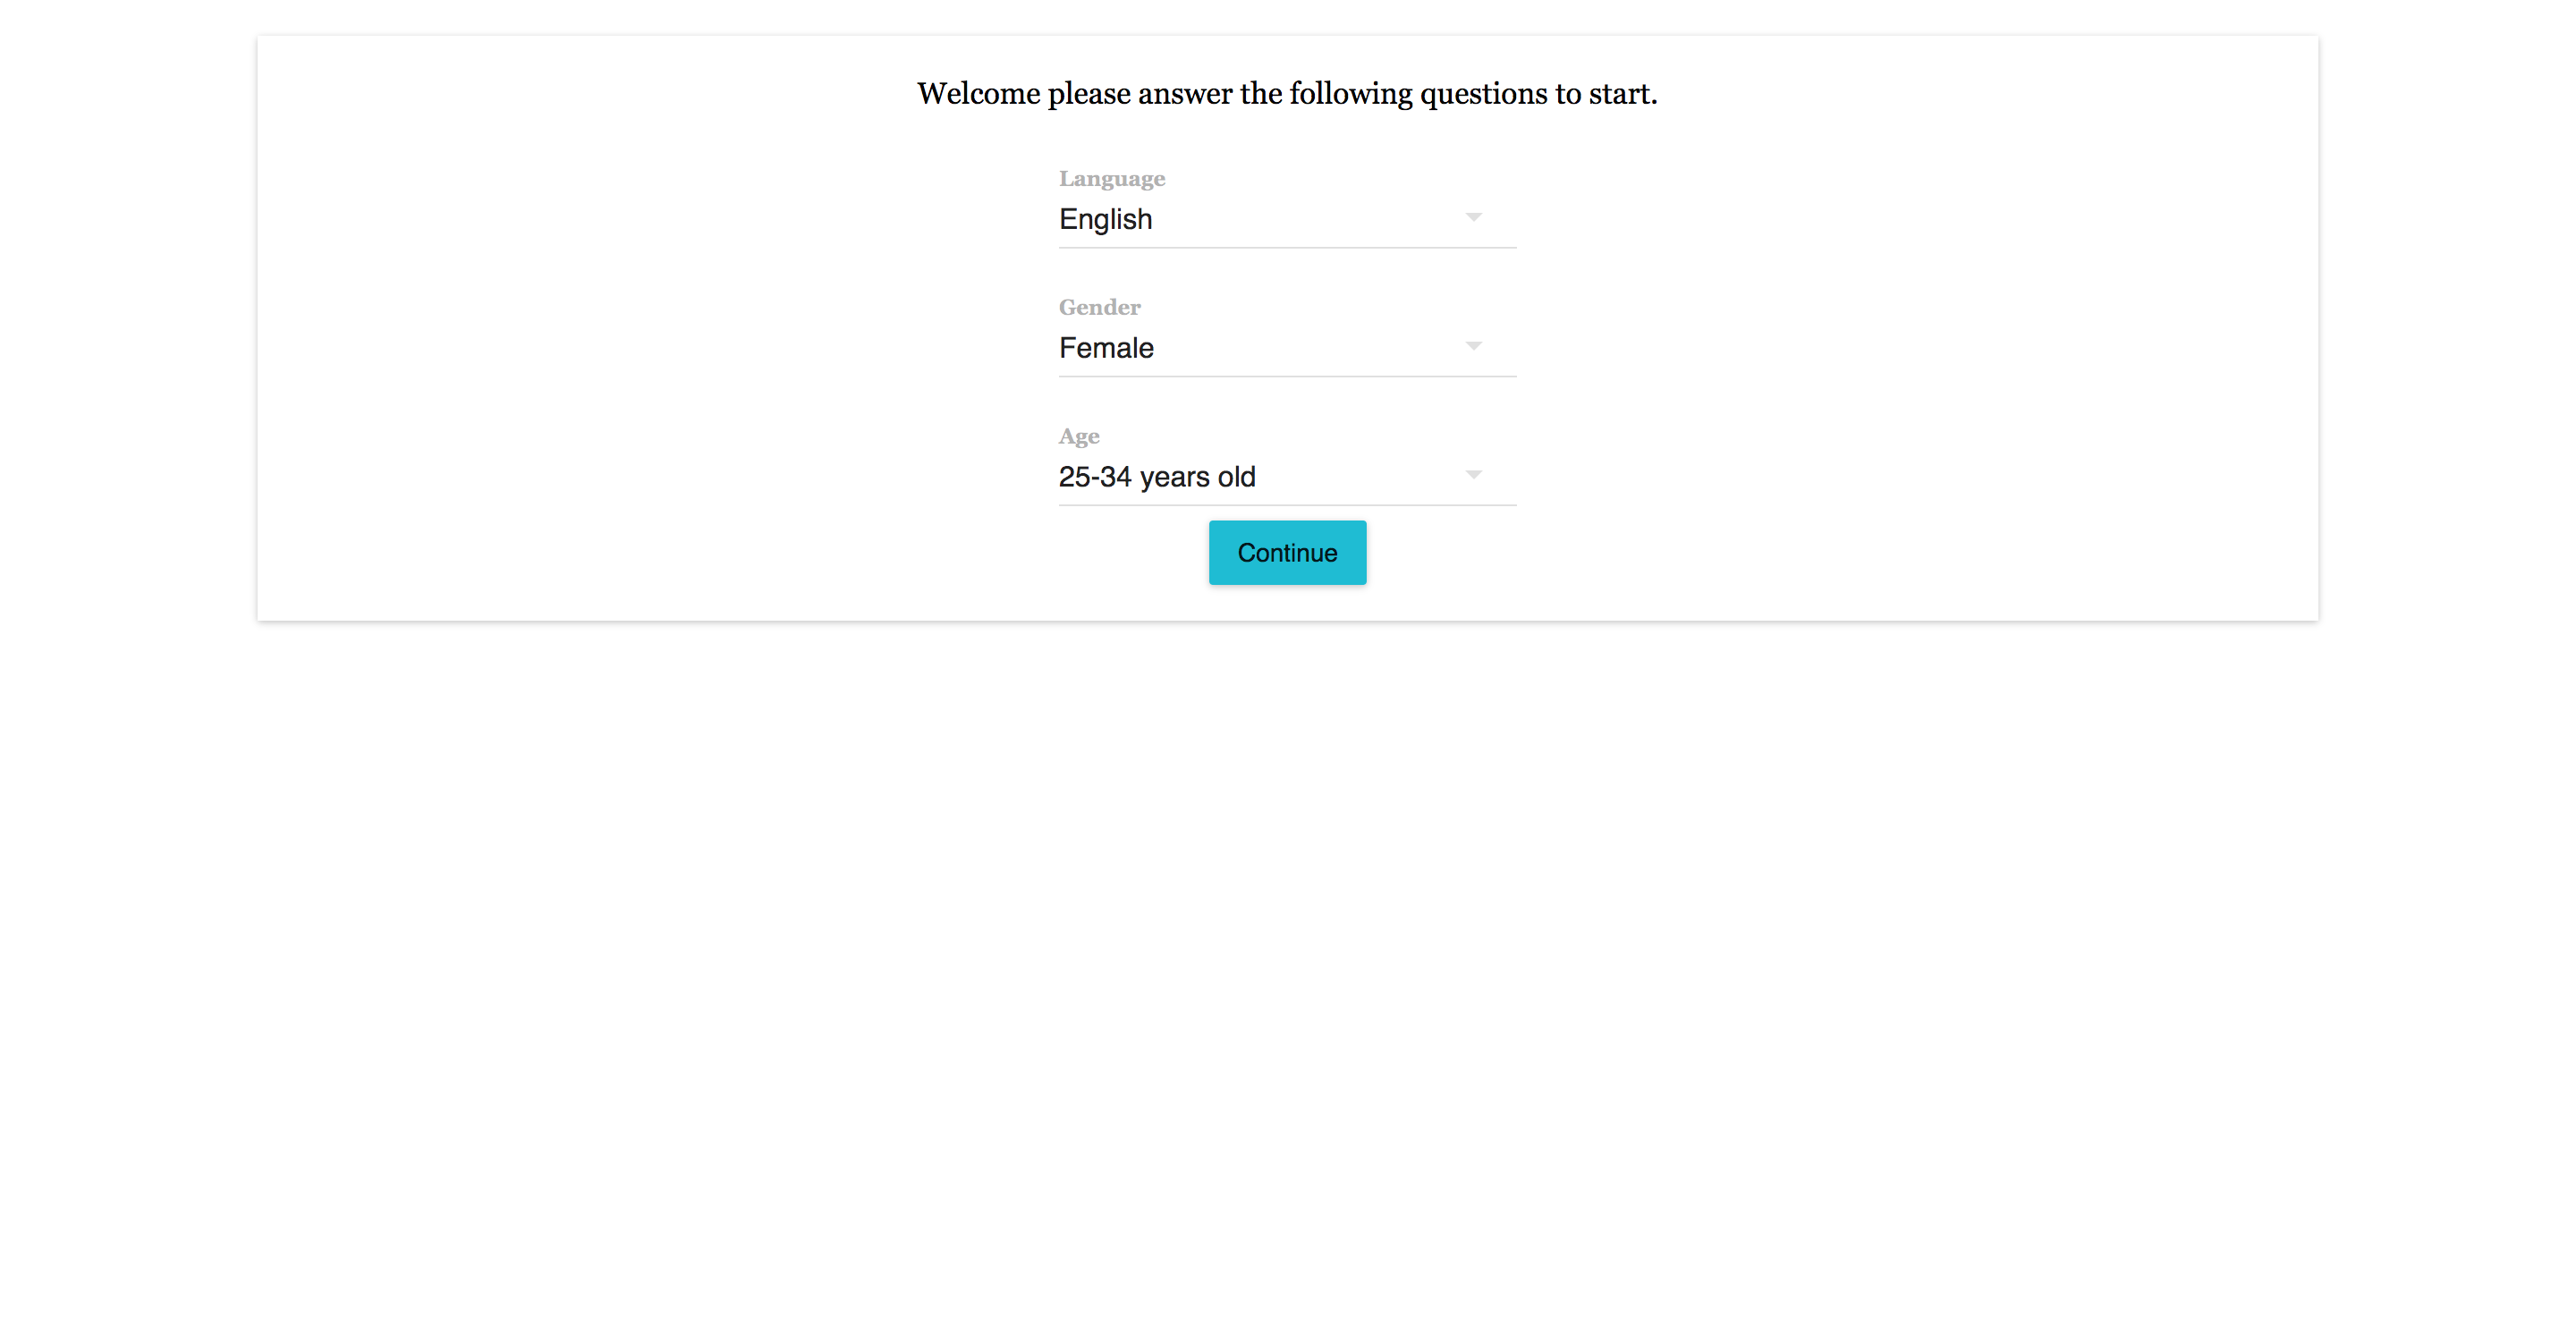
\includegraphics[width=100mm]{Images/homepage.png}
	\decoRule
	\caption[Homepage]{Image of the first page the user is greeted with. }
	\label{fig:homepage}
\end{figure}

\begin{figure}[h]
	\centering
	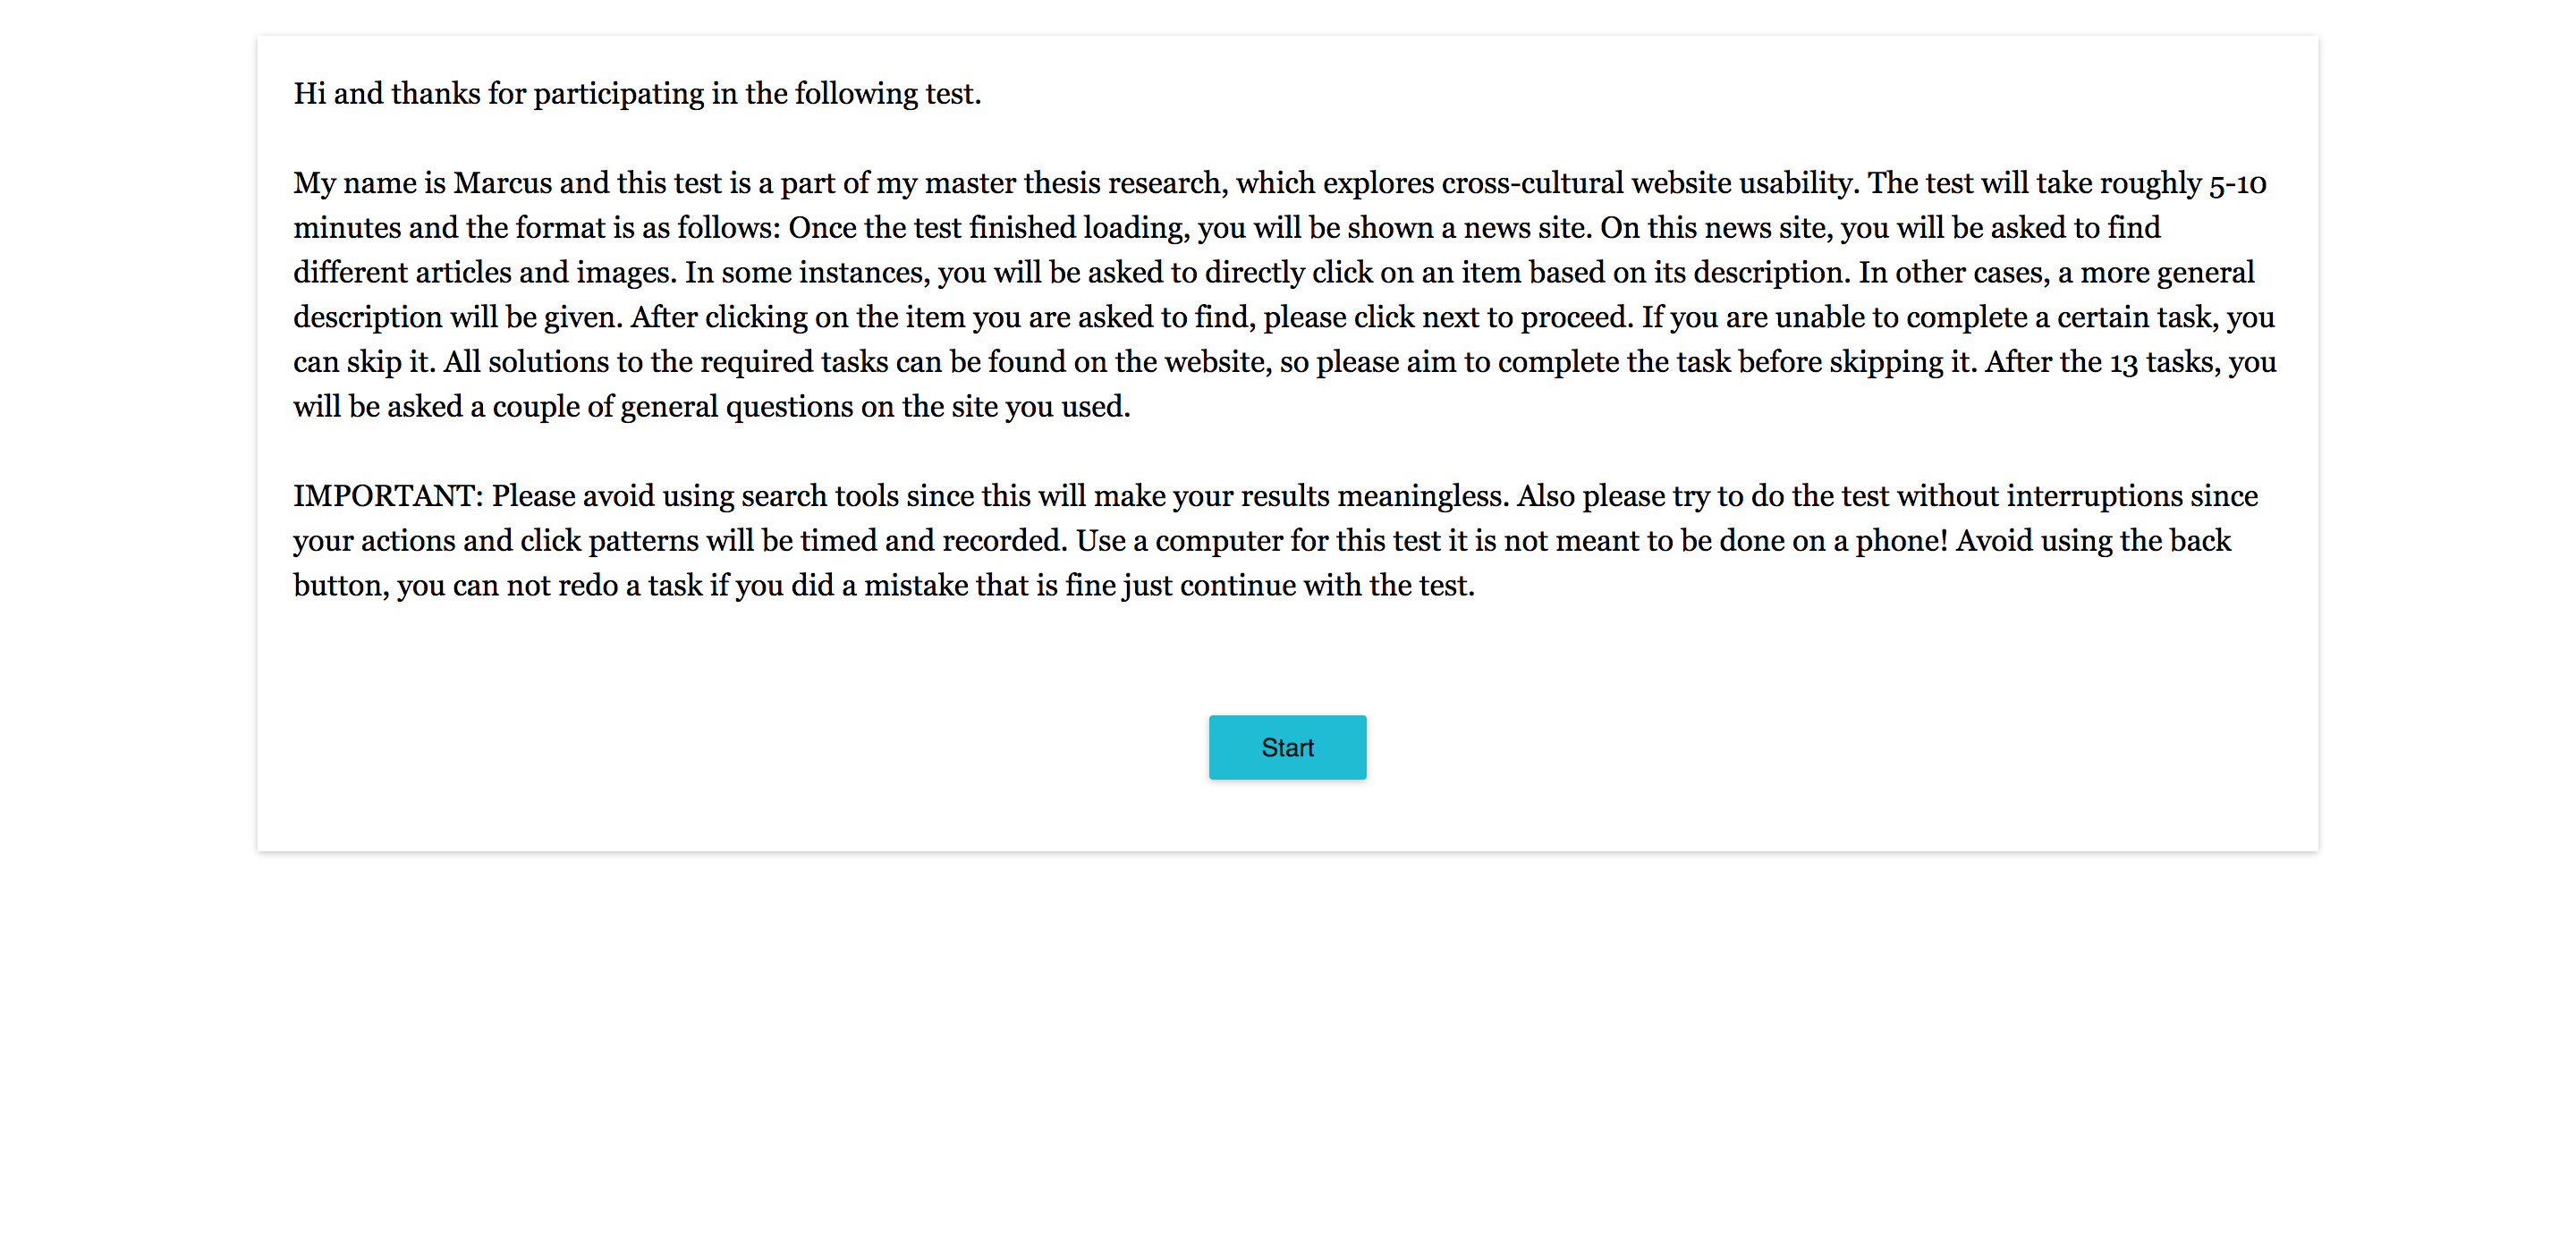
\includegraphics[width=100mm]{Images/homepage_text_en.png}
	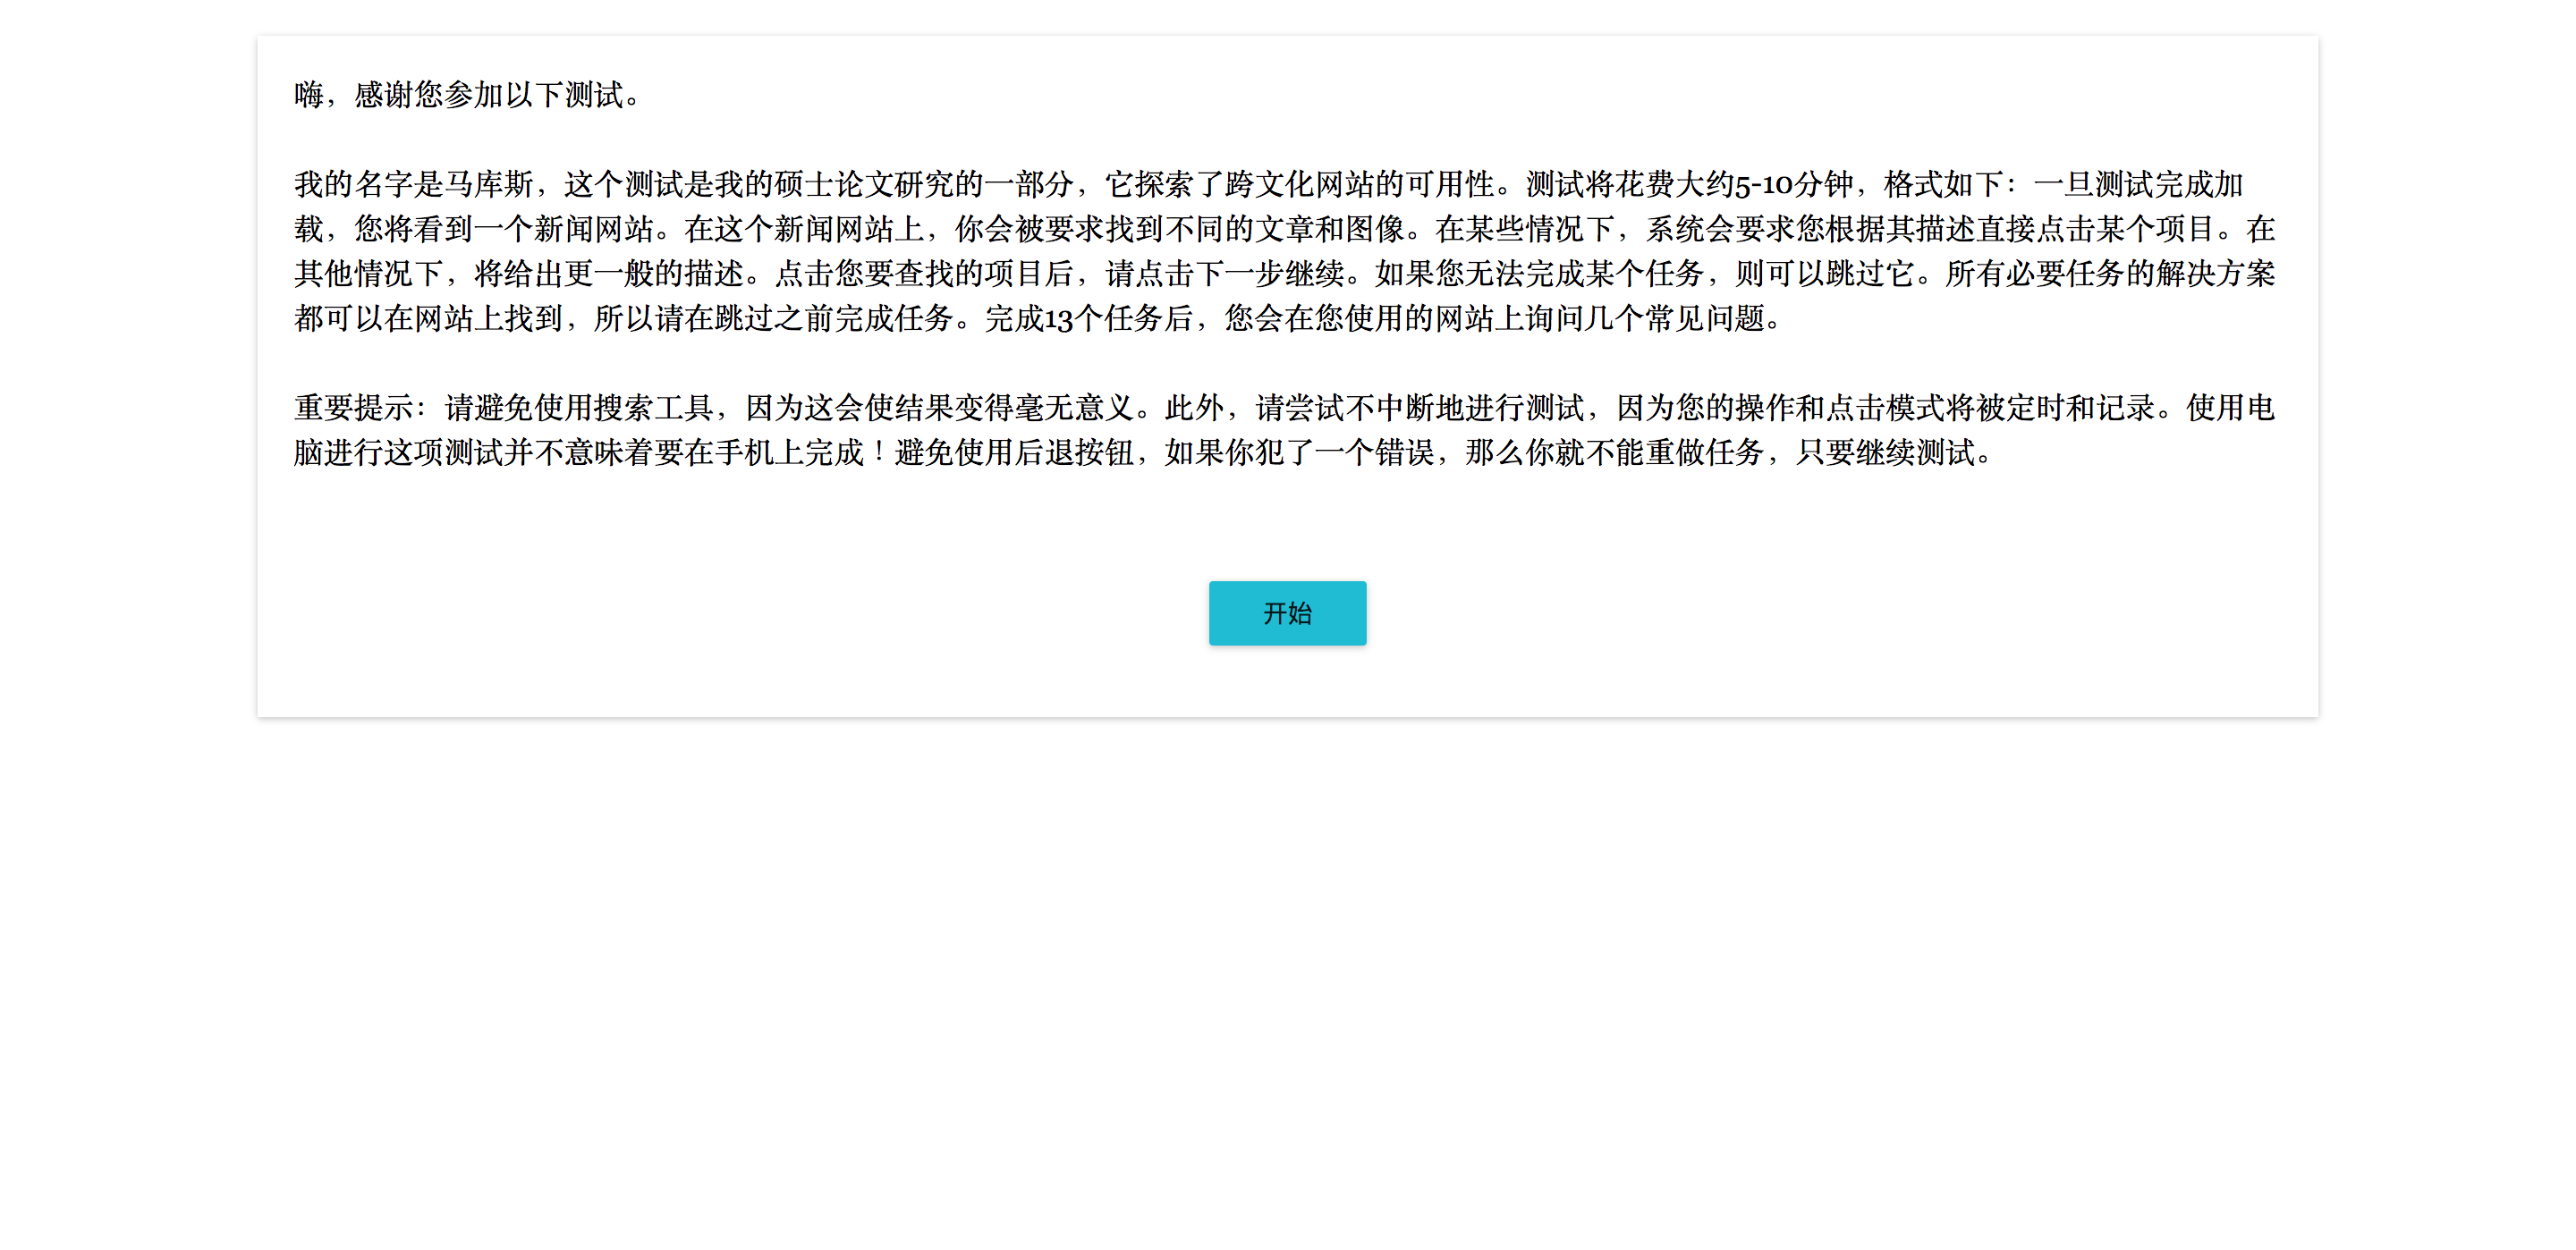
\includegraphics[width=100mm]{Images/homepage_text_zh.png}
	\decoRule
	\caption[Homepage]{Description in chinese and english.}
	\label{fig:homepage_desc}
\end{figure}
\subsubsection{BBC and QQ}
Both the bbc and qq inspired sites have the same basic layout. When the user arrives at the page a pop-up will appear with a loading bar, this is to make sure the user can't start the test until all the images has been loaded from the server. When all the images have been loaded the user will be able to start the test (see ref....).  
\\\\
All the news in this test has been translated so they have both the English and Chinese versions available depending on what language the user selected from the Homepage. Once the user starts the test a timer starts, the user is not able to see this timer. Each click the user does is recorded, the time it takes to complete the task and if the user gets the correct task or not. The number of questions the user have left to complete is also shown. The questions and what the user has most recently clicked is shown in a bar at the bottom of the screen (see \ref{fig:user_view}). Once the user finishes the test their answers are sent to the database via the API and they are redirected to the SUS site. 
\begin{figure}[h]
	\centering
	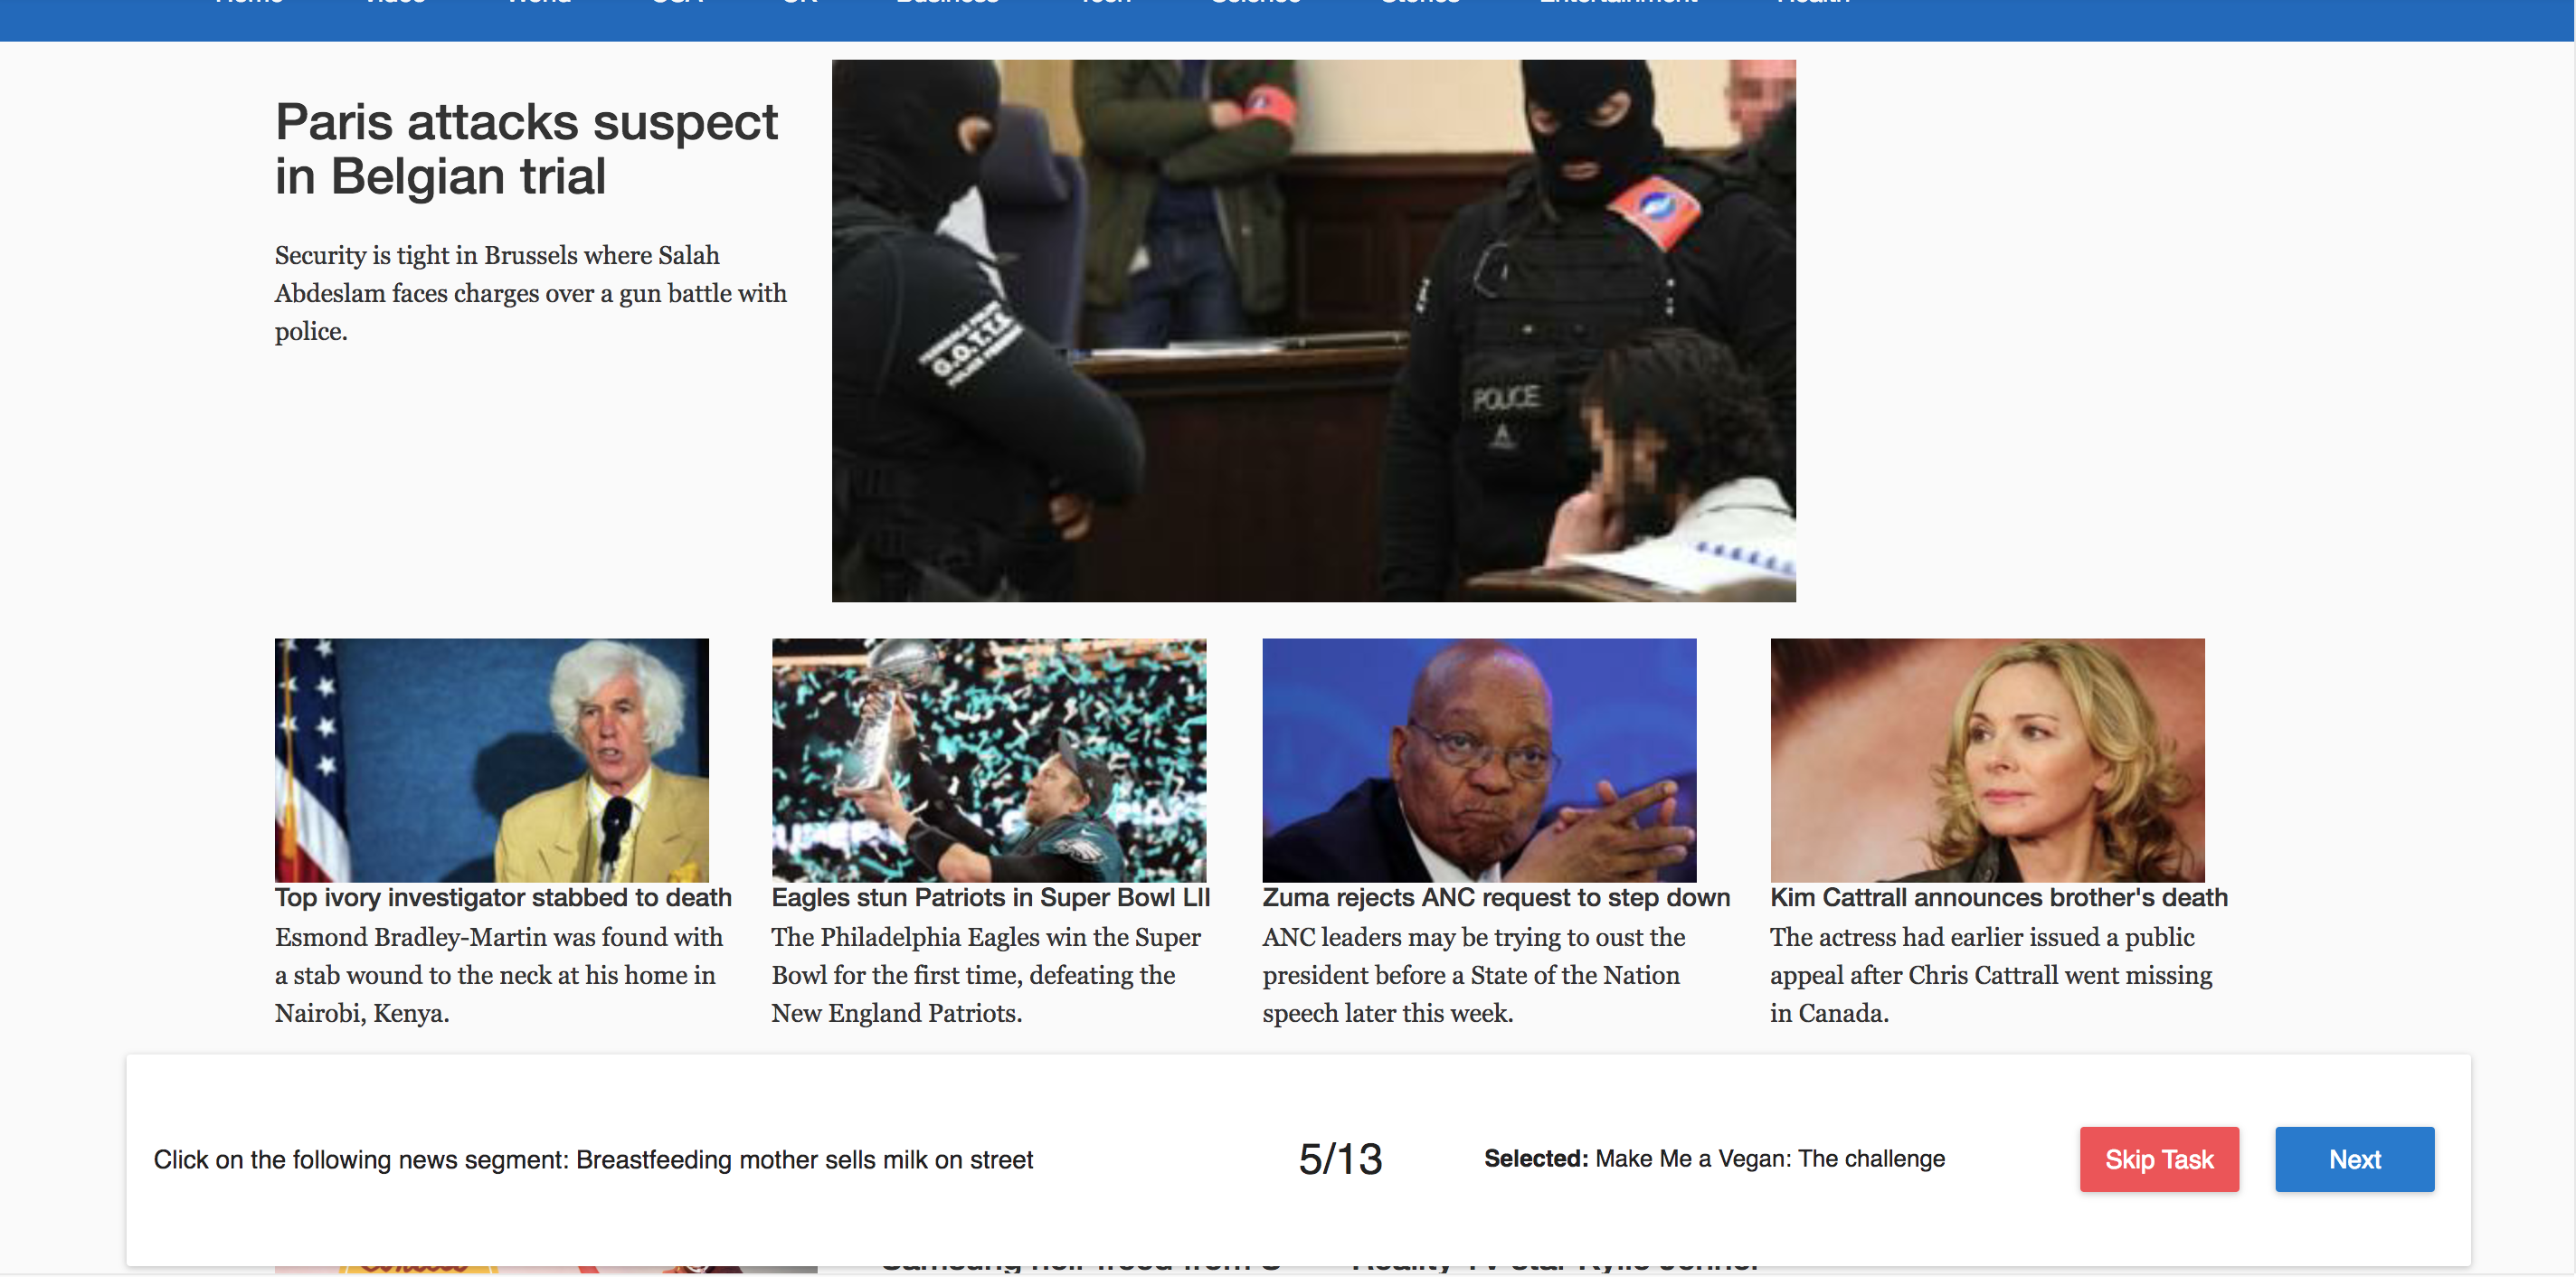
\includegraphics[width=70mm]{Images/view_bbc.png}
	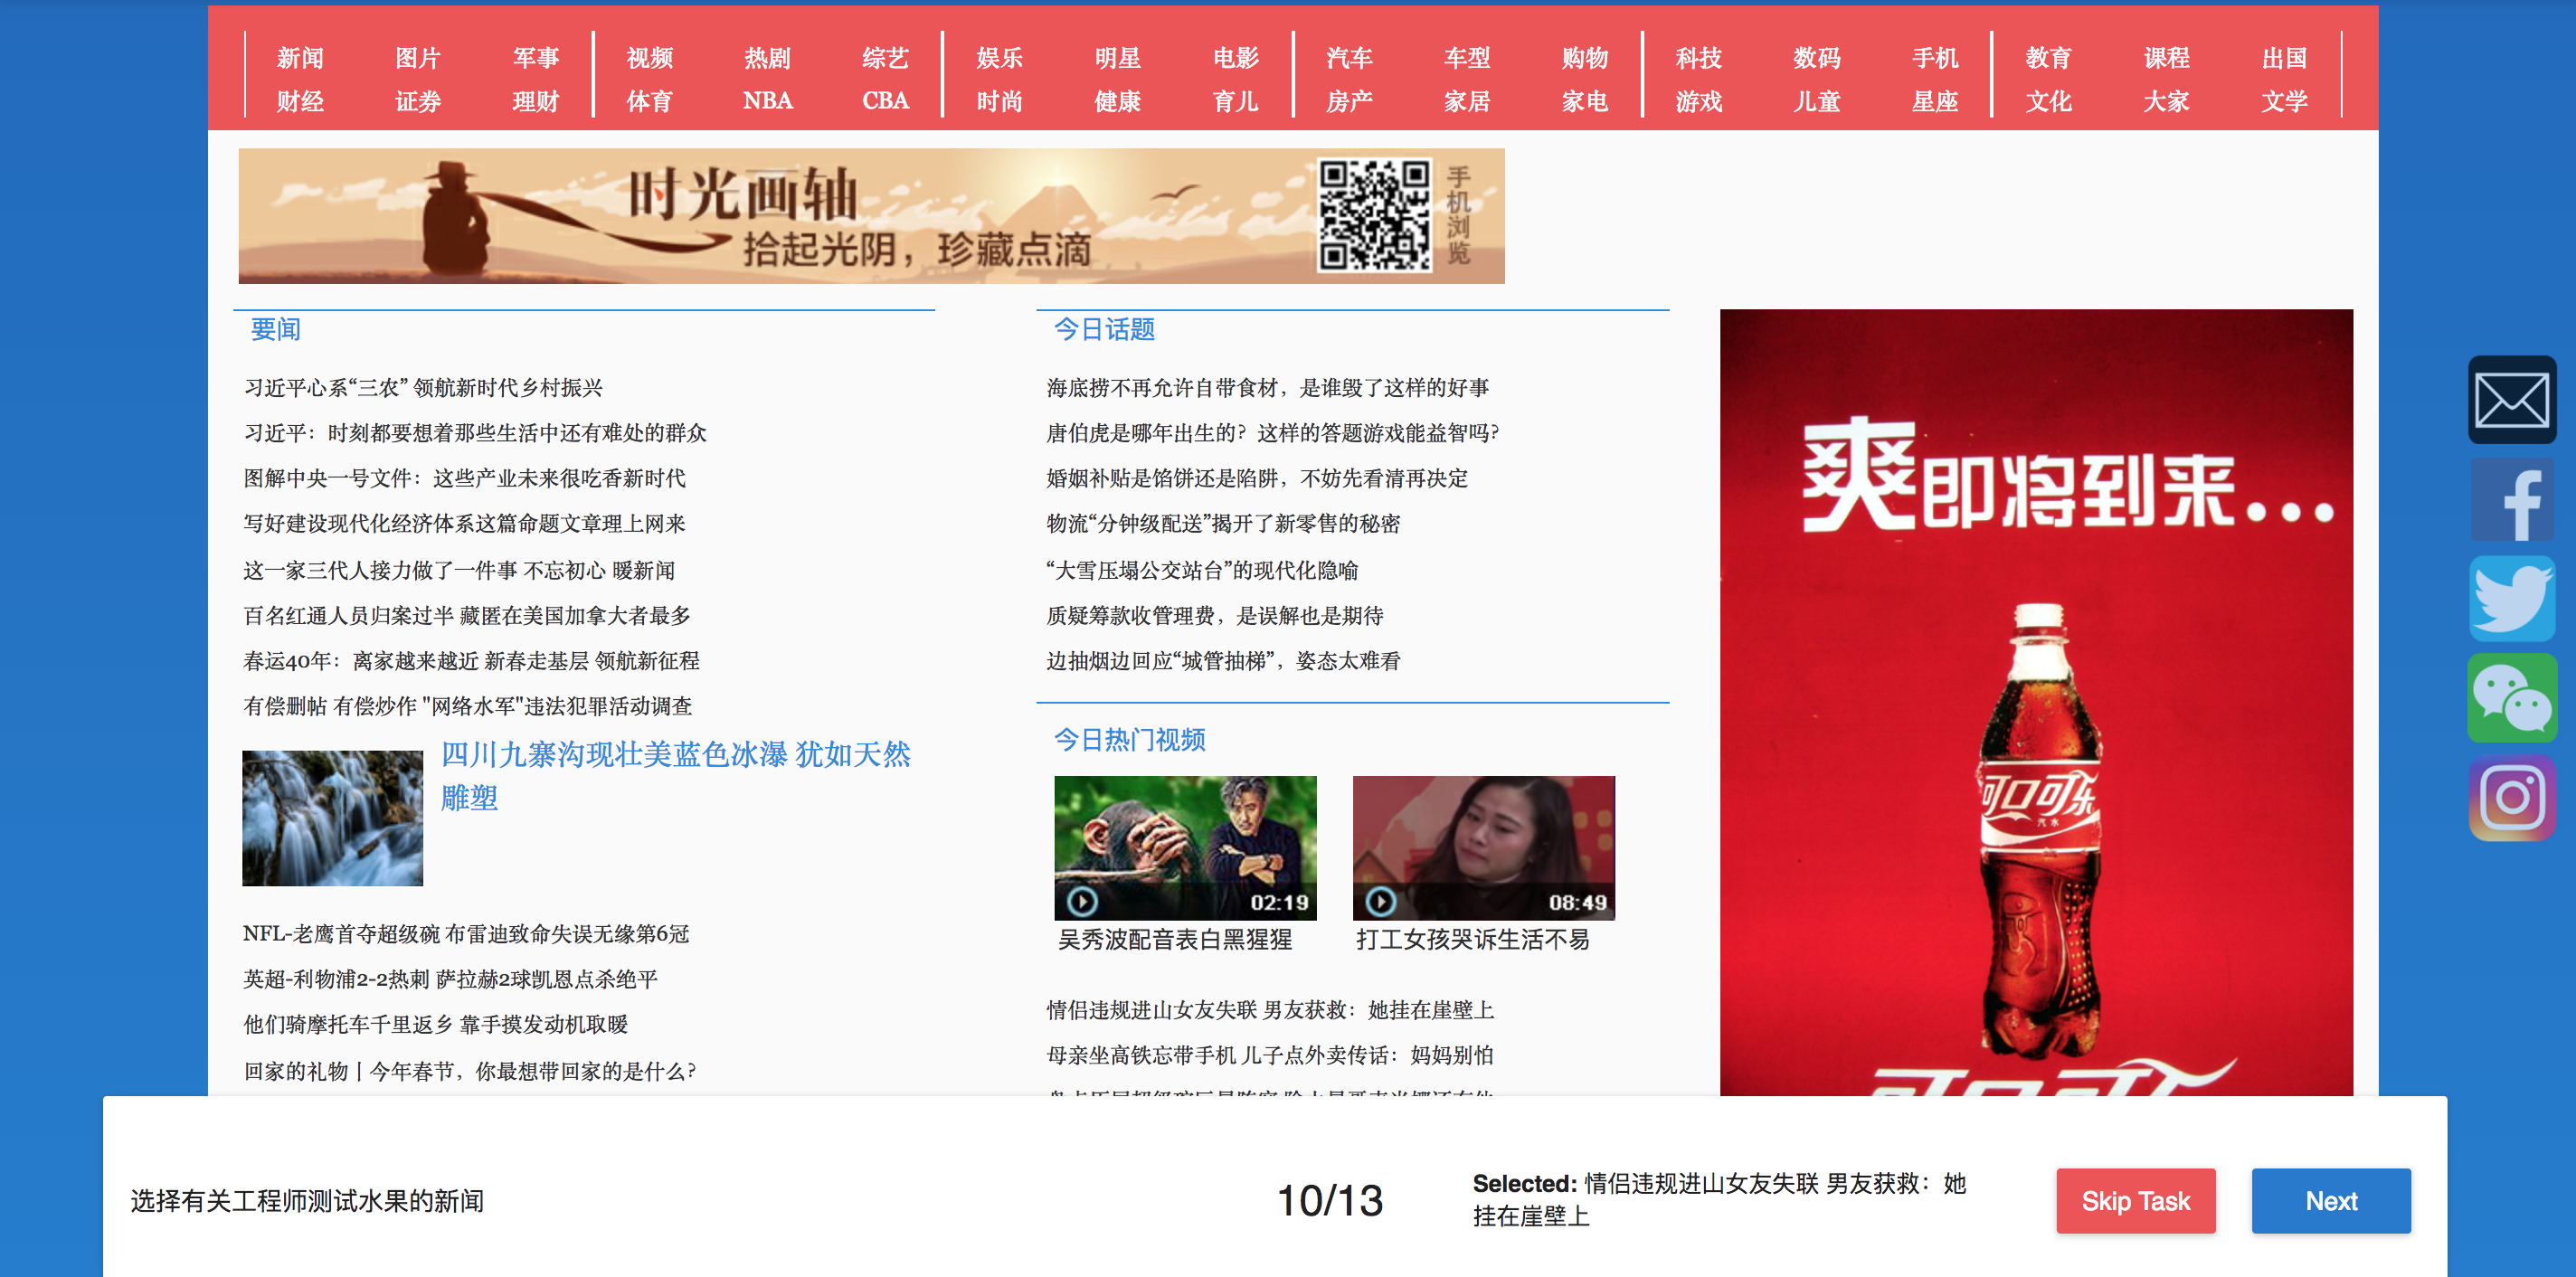
\includegraphics[width=70mm]{Images/view_qq.png}
	\decoRule
	\caption[Users View]{A example of what it might look for a user when testing bbc and qq inspired websites.}
	\label{fig:user_view}
\end{figure}
\begin{figure}[h]
	\centering
	\includegraphics[width=70mm]{Images/qq_site_zh.png}
	\includegraphics[width=70mm]{Images/qq_site_en.png}
	\decoRule
	\caption[QQ]{The full view of QQ site in english and chinese}
	\label{fig:qq_site}
\end{figure}
\begin{figure}[h]
	\centering
	\includegraphics[width=70mm]{Images/bbc_site_zh.png}
	\includegraphics[width=70mm]{Images/bbc_site_en.png}
	\decoRule
	\caption[BBC]{The full view of BBC site in english and chinese}
	\label{fig:bbc_site}
\end{figure}


\subsubsection{SUS}
This site consists of the before mentioned predefined questions designed to get a understanding for what the user fleet about the website, test and design (See fig \ref{fig:sus_site}). Once the user has answered all the questions and pressed finish their answers will be sent to the database via the api. The user will then be rerouted to the done site where they will see a message thanking them for participating in the test (See fig \ref{fig:done_site}).


\begin{figure}[h]
	\centering
	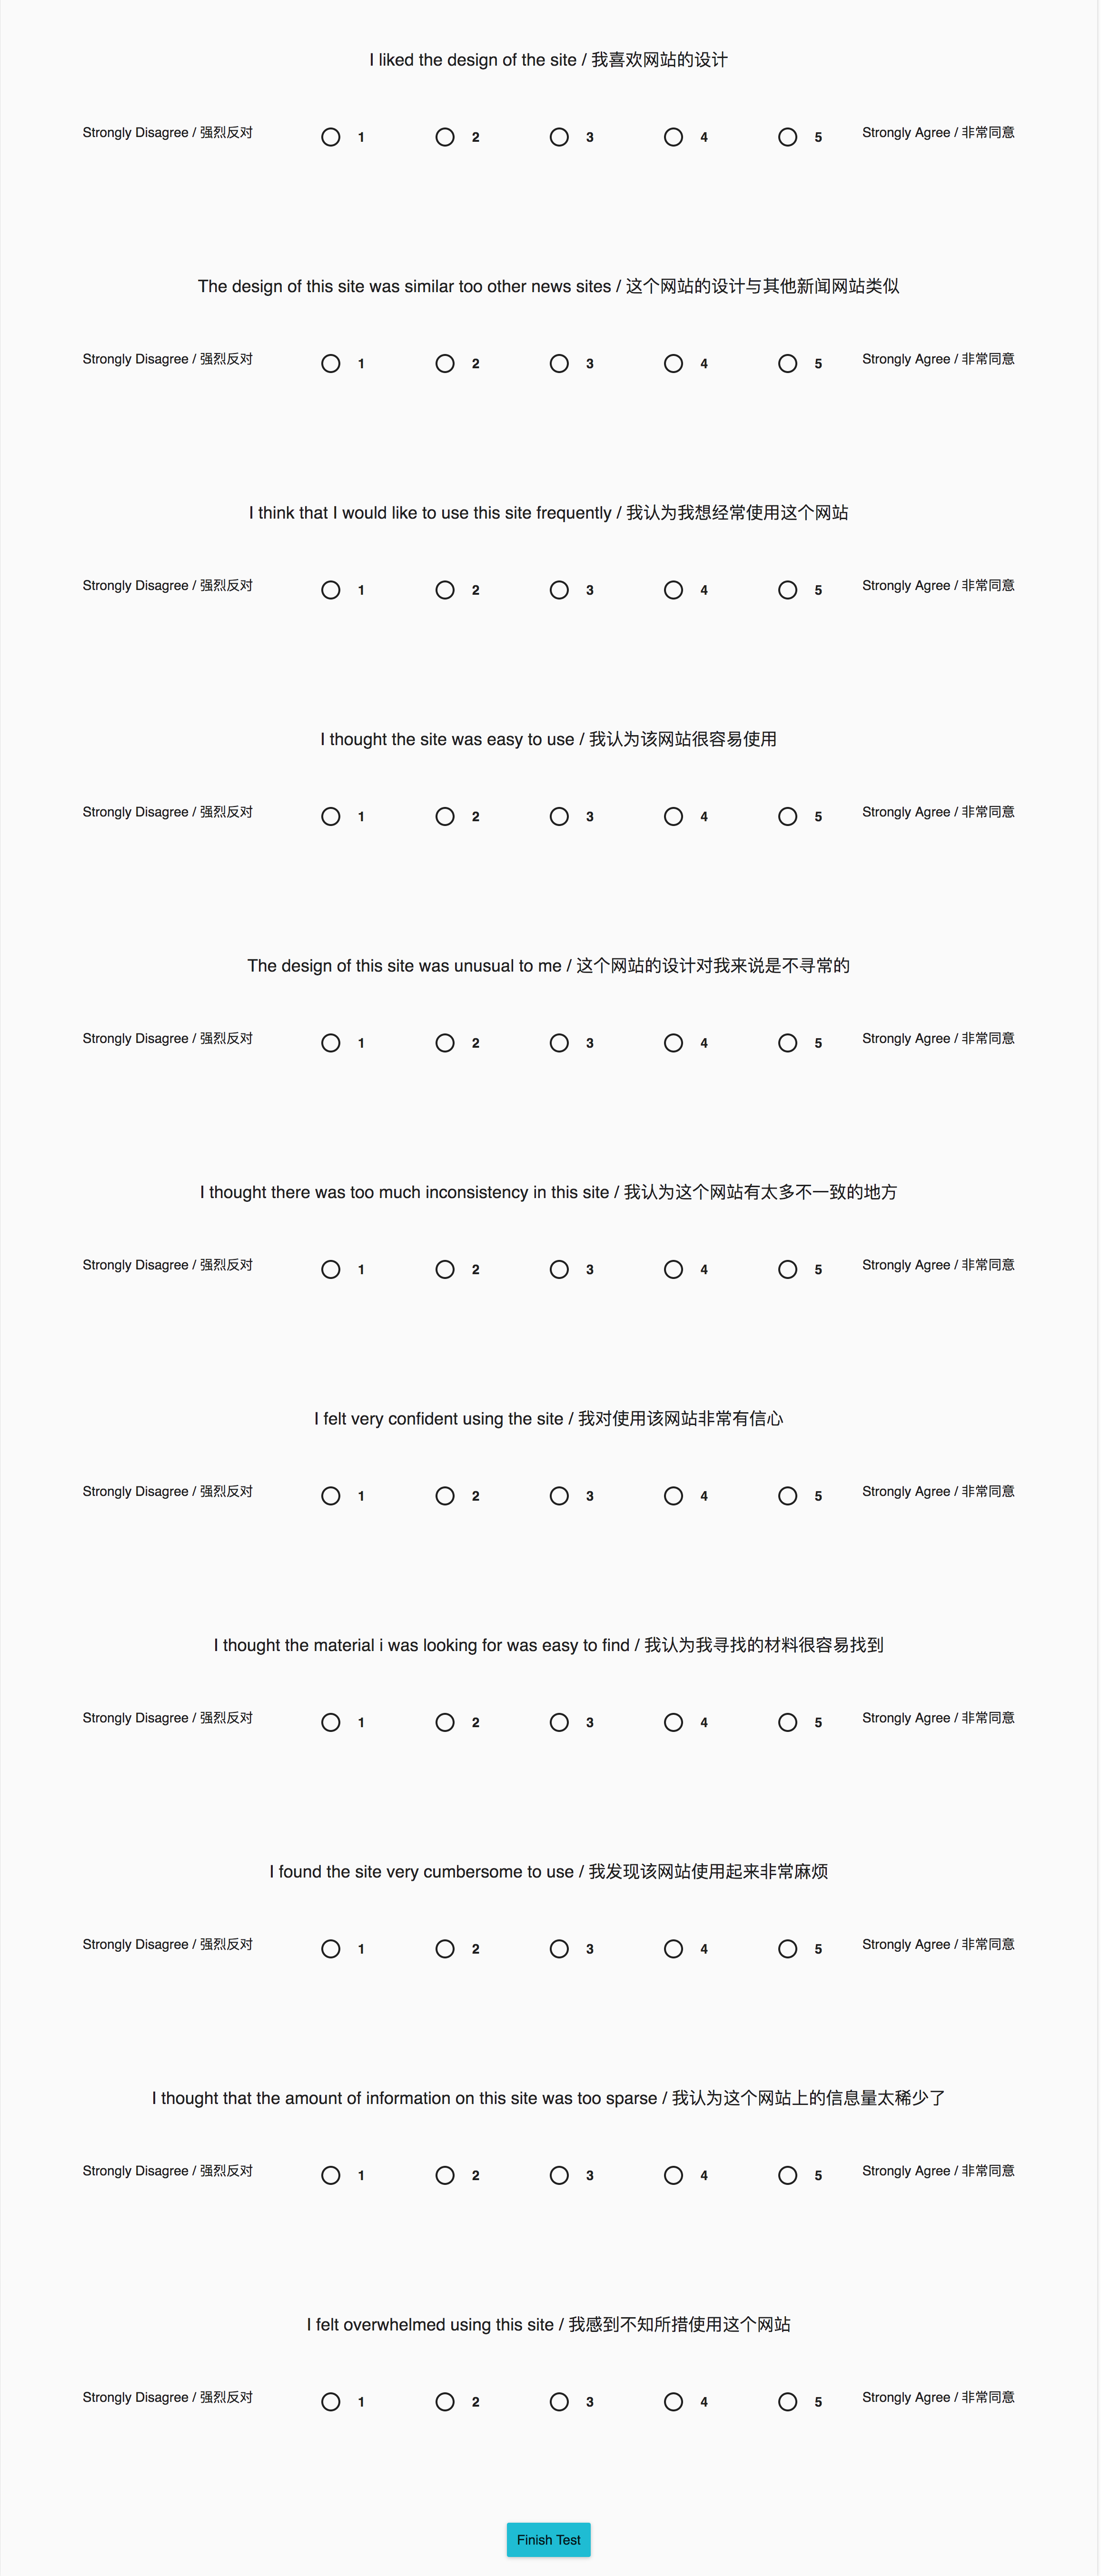
\includegraphics[width=70mm]{Images/sus.png}
	\decoRule
	\caption[SUS]{The sus site}
	\label{fig:sus_site}
\end{figure}
\begin{figure}[h]
	\centering
	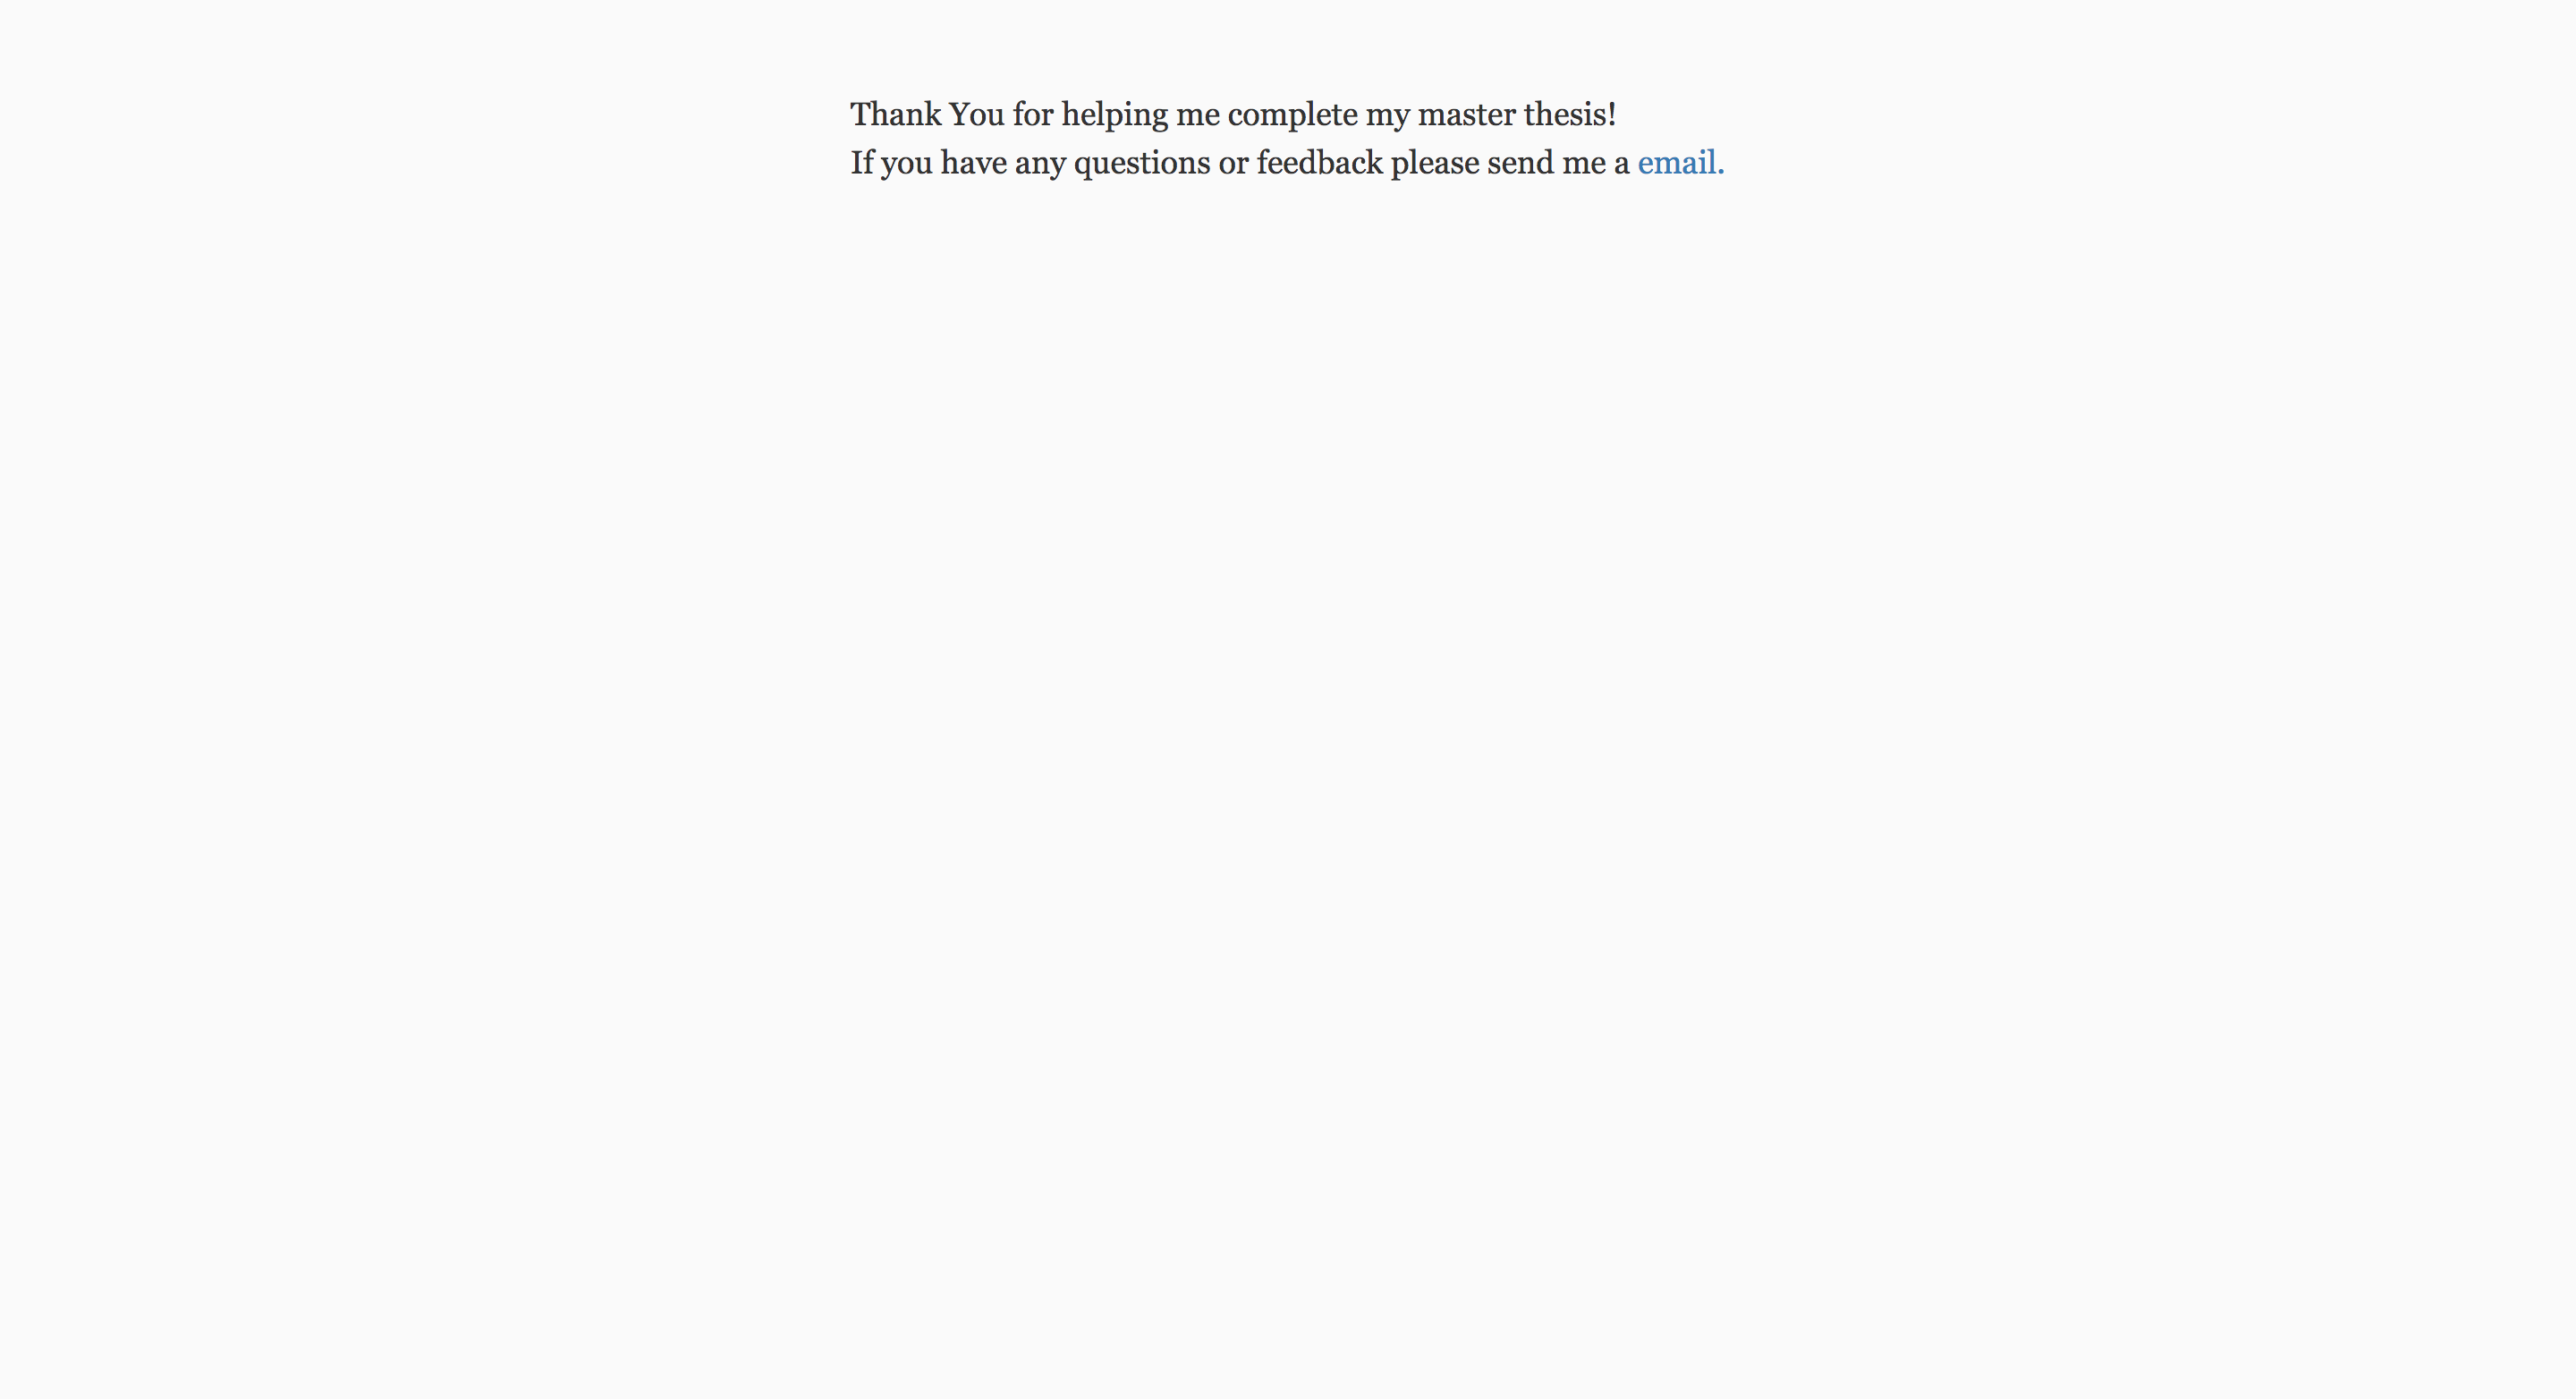
\includegraphics[width=100mm]{Images/done.png}
	\decoRule
	\caption[Done]{Last site the user is shown when they have finished the test. }
	\label{fig:done_site}
\end{figure}


\subsection{Database}
The database consists of five diffrent tables: Main, Actions, Questions, Sus and QuestionTexts. (See fig: \ref{fig:db_schema} for figure of the full database) 
\\\\
The Main mainly is used to identify the user where each user has a unique row. The table has four columns Id, Site, Language and Age. The id in the main table is the main id to identify a user. This same id can be found for each user in all other tables except QuestionTexts. 
\\\\
The Questions table contain all the answers from the users, the table has seven columns: Id, MainId, QuestionId, Correct, StartTime, EndTime, Correct, TotalTime. MainId and QuestionId is foregin keys referencing the ids in the Main and QuestionsTexts tables.
Each row in the Question table contain a answer from a user.
\\\\
The Action table contain all the click-actions a user did per question. The table contain seven columns: Id, QuestionsId, PosX, PosY, ScreenWidth, ScreenHeight, RelativeTime. Where QuestionsId is a foregin key referencing the Id in Questions. Each row in the Action table contain a action made by the user.
\\\\
The Sus table simply contains all the users answers to the Sus questions. The QuestionTexs table contain all the questions the user are asked in the test

\begin{figure}[h]
	\centering
	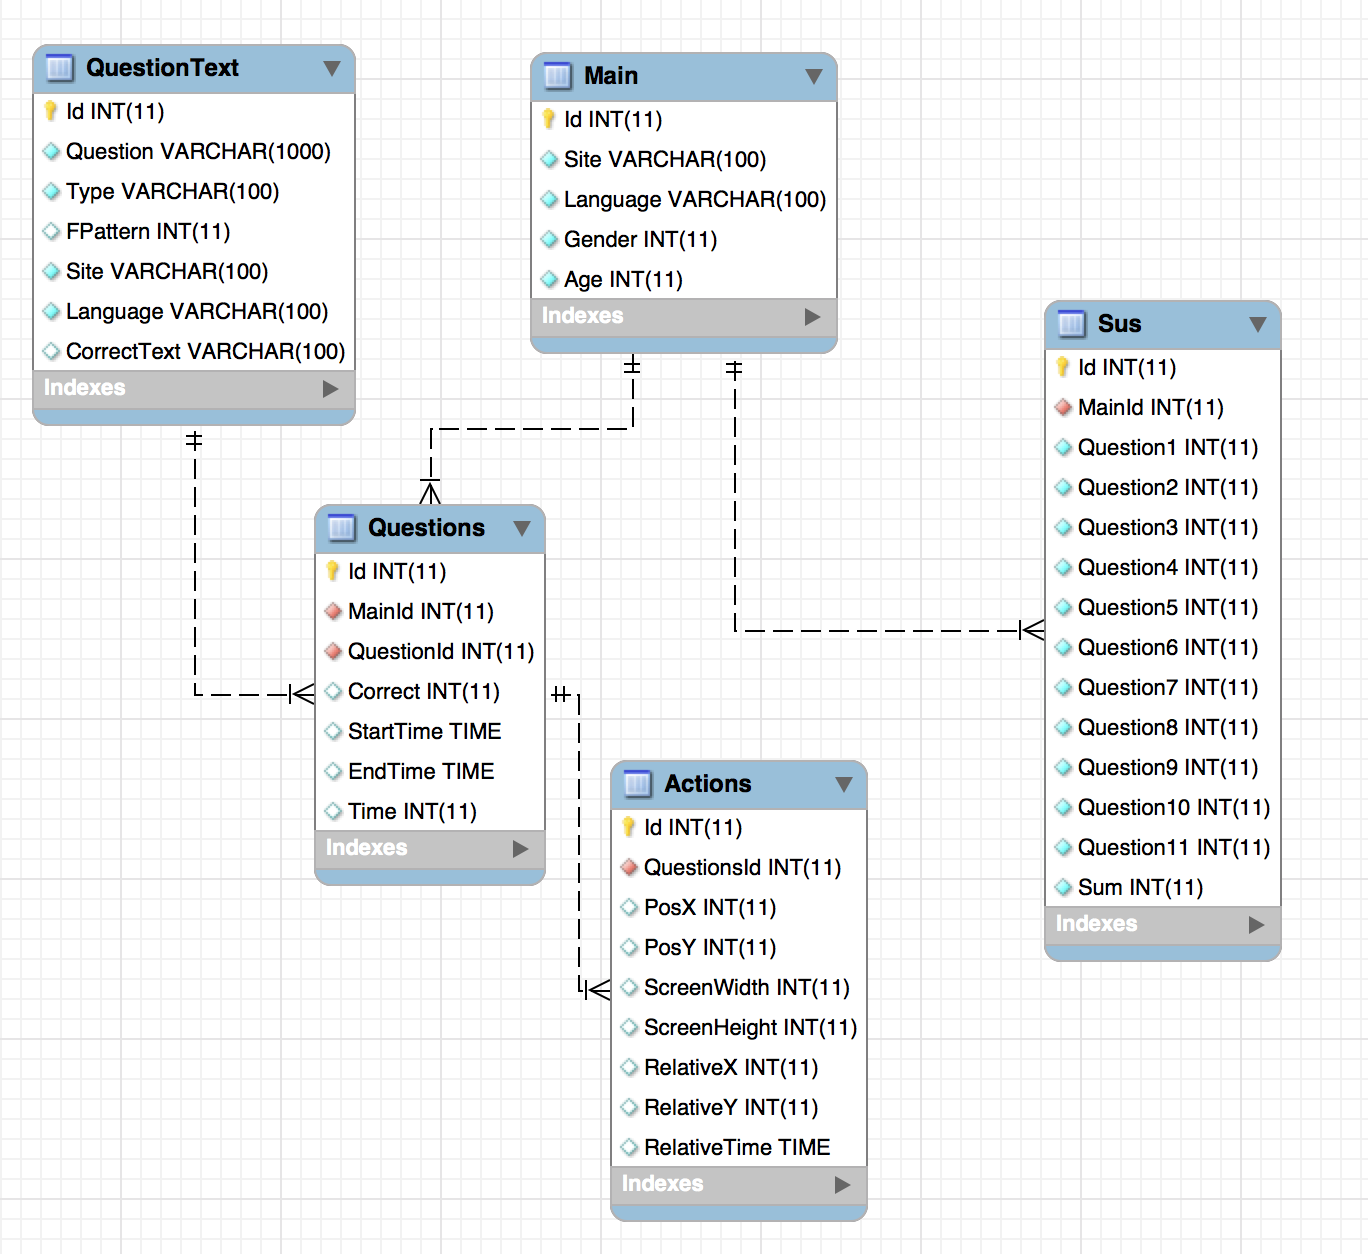
\includegraphics[width=100mm]{Images/db_eer.png}
	\decoRule
	\caption[Database Schema]{A EER schema of the mysql database. Yellow icons show the tables primary key, red the foreign keys and blue/white the atributes.}
	\label{fig:db_schema}
\end{figure}

\subsection{Api}
A express Api was set up to handle communication between the front-end and database. The Api takes the information that is sent from the users front-end code and transform it into a format that works for the sql database. The Api then quires the database and insert the new data into the database tables.

\subsection{Hosting AWS}
To host this app on AWS we used the feature called "Elastic Beanstalk" also called eb. Eb allowed us to easily launch a application that automatically set up a EC2 instance, auto scaling, load-balancing, RDS. The services was set up in Seoul. This to decrease the loading time for China as much as possible. Since Seoul also have very good network connections to the rest of the world this does not increase the loading time in Europe and the US that much. A lot of time had to be spent changing parts of the code so it would run on AWS servers.

\subsection{Beta-tests}
Once a working version of the test was created. A beta test was made to find possible bugs in code and improve user-experience in terms of font-size and design of the testing parts.
The beta-tests where made in the form of letting users try to finish the test while It was supervised. Notes where taken about possible misunderstandings, bugs and improvements that could be made to the test. Some examples of notes that was taken during the beta tests can be seen below. 

\begin{enumerate}
	\item Make selected bigger so the user can easier see what they have done.
	\item Should we log scrolling?
	\item Some correct question gets logged as incorrect in database in-spite of being correct.
	\item Waiting for sus site is very slow. Is it waiting for the database?
	\item Left top-side of qq site is too small, because of commercial?
	\item Wrong spelling in some news.
	\item Skip task not working.
	\item Some correct question gets loged as incorrect in database in-spite of being correct.
	\item Change so the size of the page is constant no matter the screen size. (Looked very bad on a big screen right now.)
	\item Start time not working correctly on some questions.
	\item Remove video from questions, does not give any relevant information.
\end{enumerate}

The beta was tested on about ten people where six did the English version of the test and four the Chinese version. After about eight tests almost no new information about usability problems and bugs where found so it was concluded to finish the beta testing and launch the test.

\subsection{Launch}
The launch of the test when fairly quickly with AWS. During the launch the performance of the site was monitored closely and we could thereby see that loading times increased when several people used the site at the same time and not all results where logged in the database. It was quickly concluded this was beacuse a problem with the database connection from the api and within the matter of minutes this bug was fixed and the site was updated. It can be estimated that about 4-5 test results where lost due to this mistake.

\subsection{How the test was conducted}
it was sent out so only one test person did the test once. No repeats of the test where made

\section{Results} (CHANGE)
We received quite a few responses from both English and Chinese users. In total we revived about 99 replies from people who did the test. 40 of these where from Chinese users and 59 from English speaking users. Of these users 61 where male and 38 female.  
 
 The majority of the test subjects are students studying at university. Most of the english speaking students are from Lunds University and the majority of the Chinese speakers are from xxxxx university in China. The rest of the test subjects are a mix of people from the Swedish and Chinese Tetra pak offices.
 The age of the test subjects are quite similar as can be seen in the graph below (/ref here for graph!).
 
(Bild från age grafen)
 

\section{Discussion}
The programing is the largest and most time consuming part of this thesis and there were several requirents of the code for the tests results to be useful. (OBS BORDE DHA MED ALLA REQUIREMTENTS NÅGONSTANTS. The requirements from the code can be seen in (REF TO REQ HERE). On top of previusly decided requirements the following where also added when it was realised that they where needed: 
 \begin{enumerate}
 	\item Users are not allowed to use ctrl-search
 	\item What site the user will test on should be controlled, this so we receive equal amount of tests for both sites.
 	\item 
 \end{enumerate}

The results are from the raw data. This means that the data will have to be cleaned before able to be used. Some examples of what have to be removed are: 

\begin{enumerate}
	\item Tests done on Phone
	\item Questions where the user has left the test.
	\item Tests where the user only skipped through all the questions
\end{enumerate}






\section{Conclusion}
Vad som behövde ändras efter beta, samt panik updatering på mysql databasen, hur vissa trots text försökte göra på mobil
